%----------------------------------------------------------------------------------------
%    PACKAGES AND THEMES
%----------------------------------------------------------------------------------------
\documentclass[aspectratio=169,xcolor=dvipsnames]{beamer}
\makeatletter
\def\input@path{{theme/}}
\makeatother
\usetheme{CleanEasy}
\usepackage[utf8]{inputenc}
\usepackage{lmodern}
\usepackage[T1]{fontenc}
% \usepackage[brazil]{babel}
\usepackage{fix-cm}
\usepackage{amsmath}
\usepackage{mathtools}
\usepackage{listings}
\usepackage{xcolor}
\usepackage{hyperref}
\usepackage{graphicx} % Allows including images
\usepackage{booktabs} % Allows the use of \toprule, \midrule and \bottomrule in tables
\usepackage{tikz}
\usetikzlibrary{positioning, shapes, arrows, calc, decorations.pathreplacing, arrows.meta, backgrounds, patterns, overlay-beamer-styles,tikzmark}
\usepackage{etoolbox}
\usepackage{tcolorbox}
\usepackage{animate}
\usepackage{xeCJK}
\setCJKmainfont{SourceHanSansSC-Regular.otf}[Path=./font/, BoldFont=SourceHanSansSC-Bold.otf, AutoFakeSlant]
\setCJKsansfont{SourceHanSansSC-Regular.otf}[Path=./font/, BoldFont=SourceHanSansSC-Bold.otf, AutoFakeSlant]
\usepackage{caption}
\captionsetup[table]{labelformat=empty}
\captionsetup[figure]{labelformat=empty}
\usepackage{tcolorbox}

% \linespread{1.3}  % 行距倍数（需 \selectfont）

\AtBeginSection{}
%----------------------------------------------------------------------------------------
%    LAYOUT CONFIGURATION
%----------------------------------------------------------------------------------------
\input{configs/configs}
%----------------------------------------------------------------------------------------
%    TITLE PAGE
%----------------------------------------------------------------------------------------


%---------------------------------------------


\title[]{基于Hu-Washizu变分原理的薄壳结构 \\ 准变分一致无网格法}

\author[]{吴俊超}

\institute[HQU]{
华侨大学土木工程系
\and
福建省智慧基础设施与监测重点实验室（华侨大学）
}


\vspace{-2cm}\date{2026年8月}
% Define positions for logos on title page
\titlegraphic{
  \begin{tikzpicture}[remember picture, overlay]
    
    \node[anchor=north west] at (current page.south west) {
    第五届无网格粒子类方法进展与应用研讨会
    };

    % 
    % \node[anchor=south west, xshift=2.5cm, yshift=0cm] at (current page.south west) {
      % 
\includegraphics[height=0.9cm]{logos/CleanEasy-logo2.png}
    % };
    
    % 
    \node[anchor=north east, xshift=-0.8cm, yshift=-0.3cm] at (current page.north east) {
      
\includegraphics[height=1.1cm]{logos/logo2.pdf}
    };
    
    %
    % \node[anchor=north east, xshift=-2.8cm, yshift=-0.3cm] at (current page.north east) {
      % 
\includegraphics[height=1.4cm]{logos/logo1.pdf}
    % };
  \end{tikzpicture}
}


%----------------------------------------------------------------------------------------


\begin{document}

\begin{frame}[plain]
  \titlepage
\end{frame}

\begin{frame}[plain]{目录}
  \tableofcontents
\end{frame}

\section{薄壳结构伽辽金无网格法}

\begin{frame}{薄壳结构控制方程}

\begin{columns}
    \column{0.45\textwidth}
        \textbf{壳体中面应变与曲率}
        \begin{equation*}
            \begin{aligned}
                \epsilon_{\alpha\beta} &= \frac{1}{2}(\boldsymbol a_\alpha \cdot \boldsymbol u_{,\beta} + \boldsymbol u_{,\alpha}\cdot \boldsymbol a_\beta) \\ 
                &= \varepsilon_{\alpha\beta} + \kappa_{\alpha\beta}\xi^3 \\
            \end{aligned}
        \end{equation*}
        \textbf{Kirchhoff假设}
        \begin{equation*}
            \epsilon_{3i} = 0 \Rightarrow
            \Rightarrow \boldsymbol \theta = - \boldsymbol u_{,\alpha} \cdot \boldsymbol a_3 \boldsymbol a^\alpha
        \end{equation*}
        \vspace{-25pt}
        \begin{center}
            \tikz{\node[
                single arrow, draw,
                fill=MediumBlue,
                minimum width=0.1cm,
                minimum height=0.7cm,
                single arrow head extend=0.2cm,
                % single arrow tip angle=60,
                shape border rotate=270,
            ] {};}
        \end{center}
        \vspace{-15pt}
        \textbf{薄壳结构曲率}
        \begin{align*}
            \varepsilon_{\alpha\beta} &= \frac{1}{2}(\boldsymbol a_\alpha \cdot \boldsymbol u_{,\beta} + \boldsymbol u_{,\alpha}\cdot \boldsymbol a_\beta) \\
            \kappa_{\alpha\beta} &= (\Gamma^\gamma_{\alpha\beta}\boldsymbol u_{,\gamma} - \alert{\boldsymbol u_{,\alpha\beta}}) \cdot \boldsymbol a_3 = - \boldsymbol u_{,\alpha}\vert_\beta \cdot \boldsymbol a_3
        \end{align*}


    \column{0.5\textwidth}
        \begin{figure}
            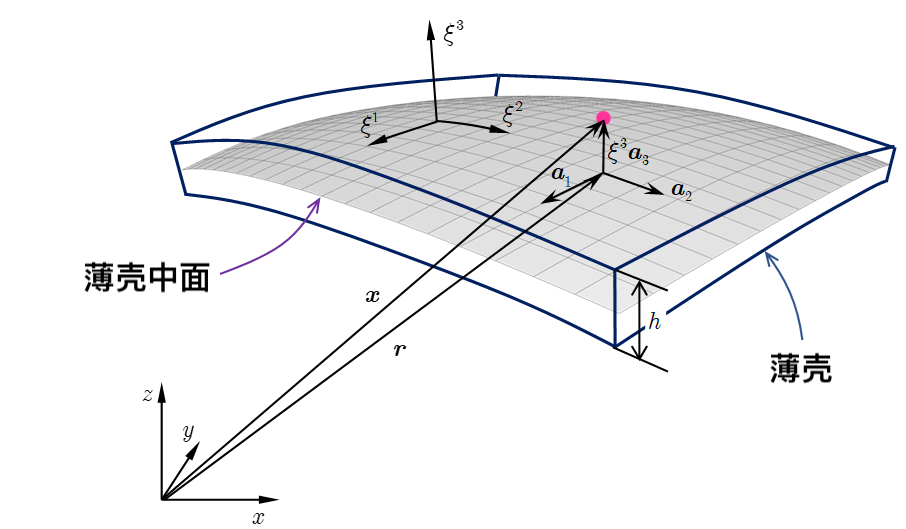
\includegraphics[width=\textwidth]{figures/1.png}
            \caption{\bfseries 薄壳结构中面}
        \end{figure}
        \begin{tcolorbox}[colback=red!5, colframe=red!75!black,left=5pt,right=5pt]
            \bfseries 薄壳结构分析曲率近似需要高阶形函数
        \end{tcolorbox}
\end{columns}

\end{frame}

\begin{frame}{再生核无网格近似}
\begin{columns}
    \column{0.45\textwidth}
        \textbf{位移近似}
        \begin{equation*}
            \boldsymbol u^h(\boldsymbol \xi) = \sum_{I=1}^{n_p} \Psi_I(\boldsymbol \xi) \boldsymbol d_I
        \end{equation*}
        \begin{equation*}
            \Psi_I(\boldsymbol \xi) = \boldsymbol p^T(\boldsymbol \xi)\boldsymbol c(\boldsymbol \xi) \phi(\boldsymbol \xi_I - \boldsymbol \xi)
        \end{equation*}
        \textbf{一致性条件}
        \begin{equation*}
            \begin{aligned}
            &\sum_{I=1}^{n_p} \Psi_I(\boldsymbol \xi)\boldsymbol p(\boldsymbol \xi_I) = \boldsymbol p(\boldsymbol \xi) \\
            \Rightarrow &
            \boldsymbol c(\boldsymbol \xi) = \boldsymbol A^{-1}(\boldsymbol \xi)\boldsymbol p(\boldsymbol 0)
            \end{aligned}
        \end{equation*}
        \textbf{无网格形函数}
        \begin{equation*}
            \Psi_I(\boldsymbol \xi) = \boldsymbol p^T(\boldsymbol \xi_I-\boldsymbol \xi) \boldsymbol A^{-1}(\boldsymbol \xi)\boldsymbol p(\boldsymbol 0)\phi(\boldsymbol \xi_I-\boldsymbol \xi)
        \end{equation*}
    \column{0.45\textwidth}
        \begin{figure}
            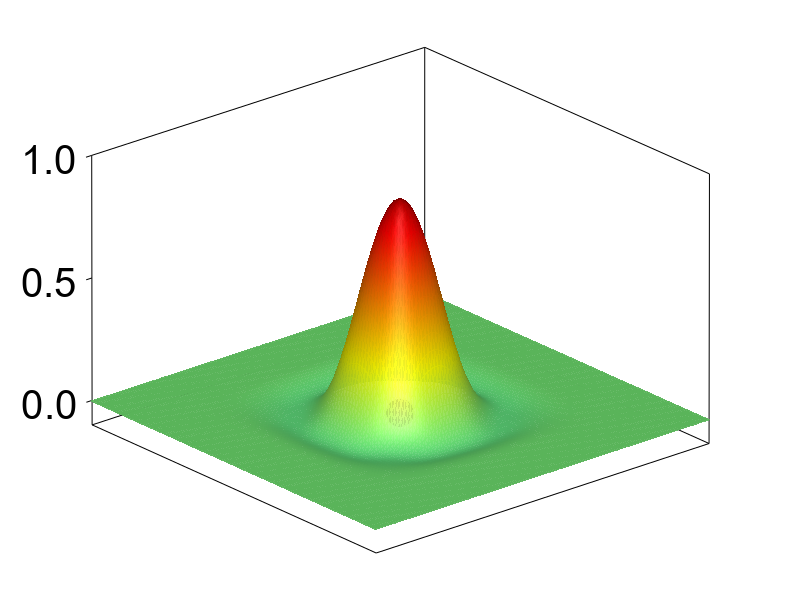
\includegraphics[width=0.7\textwidth]{figures/shape1.png}

            \vspace{-18pt}

            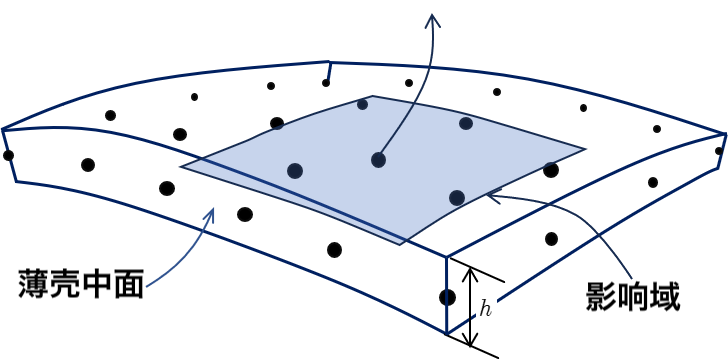
\includegraphics[width=\textwidth]{figures/3.png}
            \caption{\bfseries 再生核近似}
        \end{figure}

\end{columns}

\end{frame}

\begin{frame}{变分一致性}
\begin{columns}
    \column{0.5\textwidth}
        {\linespread{1.5}\selectfont
        \textbf{变分一致性阶次}等于伽辽金弱形式能准确求解由多项式所组成的精确解阶次:
        {\footnotesize\begin{equation*}
        \int_\Omega h \delta \varepsilon_{\alpha\beta} C^{\alpha\beta\gamma\eta} \varepsilon_{\gamma\eta}d\Omega
        +\int_\Omega \frac{h^3}{12}\delta \kappa_{\alpha\beta}C^{\alpha\beta\gamma\eta}\kappa_{\gamma\eta}d\Omega = f(\boldsymbol p^{[q]})
        \end{equation*}}
        }

    \column{0.42\textwidth}
        \begin{figure}
            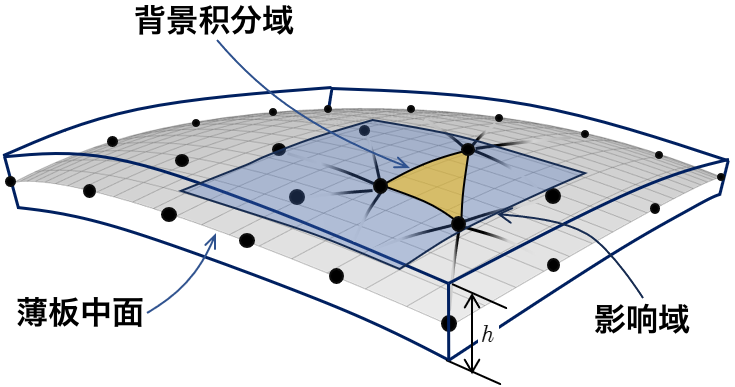
\includegraphics[width=0.9\textwidth]{figures/5.png}
            \caption{\bfseries 伽辽金无网格法数值积分}
        \end{figure}

\end{columns}

\vspace{-10pt}

\begin{tcolorbox}[colframe=MediumBlue,title=伽辽金无网格法误差估计 {\footnotesize(Wu and Wang, 2021)},height=3.4cm,valign=center]
    \begin{equation*}
    \Vert \boldsymbol u - \boldsymbol u_h\Vert_{H_e} \le \tikzmarknode[draw=red, inner sep=2pt, thick]{a}{C_p s^p\vert \boldsymbol u \vert_{H_p}} + \tikzmarknode[draw=red, inner sep=2pt, thick]{b}{C_q s^q \vert \boldsymbol u \vert_{H_q}}
    \end{equation*}
    \begin{tikzpicture}[remember picture, overlay]
        \draw[-{Stealth}, thick, red](a.south) -- ++(0,-0.3) node[below]{一致性条件控制};
        \draw[-{Stealth}, thick, red](b.north) -- ++(0,0.3) node[above]{变分一致性条件控制};
    \end{tikzpicture}

\end{tcolorbox}
\end{frame}

\begin{frame}{变分一致型边界条件施加方案}
    \begin{columns}
        \column{0.52\textwidth}
            \textbf{Nitsche法施加边界条件}

            \begin{itemize}
                \item 稳定项 \quad \uncover<2->{\alert{\footnotesize\bfseries $\times$ 人工经验参数影响求解精度}}
                    {\footnotesize\begin{equation*}
                        \begin{aligned}
                        \boldsymbol K^s_{IJ} &= \alert{\boldsymbol \alpha_v} \int_{\Gamma_v} \Psi_I \Psi_J d\Gamma 
                        + \alert{\alpha_\theta} \int_{\Gamma_\theta} \Psi_{I,\eta} n^\eta \boldsymbol a_3 \boldsymbol a_3 n^\gamma\Psi_{J,\gamma} d\Gamma \\ &+ \alert{\alpha_C} [[\Psi_I \boldsymbol a_3 \boldsymbol a_3 \Psi_J]]_{\boldsymbol x \in C_v}
                        \end{aligned}
                    \end{equation*}}
                \item 一致项 \quad \uncover<3>{\alert{\footnotesize\bfseries $\times$ 需计算形函数高阶导数}}
                    {\footnotesize\begin{equation*}
                        \begin{aligned}
                            \boldsymbol K^c_{IJ} = &- \int_{\Gamma_v} (\Psi_I \alert{\boldsymbol T_{NJ}(\Psi_{J,\alpha\beta\gamma})} + \alert{\boldsymbol T_{NI}(\Psi_{I,\alpha\beta\gamma})} \Psi_J) d\Gamma \\
                            &+ \int_{\Gamma_\theta} (\Psi_{I,\gamma} n^\gamma \boldsymbol a_3 \boldsymbol M_{\boldsymbol{nn}J} + \boldsymbol a_3 \boldsymbol M_{\boldsymbol{nn}I} \Psi_{J,\gamma}n^\gamma)d\Gamma \\
                            & + ([[\Psi_I \boldsymbol a_3 \boldsymbol P_J]] + [[\boldsymbol P_I \boldsymbol a_3 \Psi_J]])_{\boldsymbol x \in C_v}
                        \end{aligned}
                    \end{equation*}}

            \end{itemize}
        \column{0.40\textwidth}
            \begin{figure}
                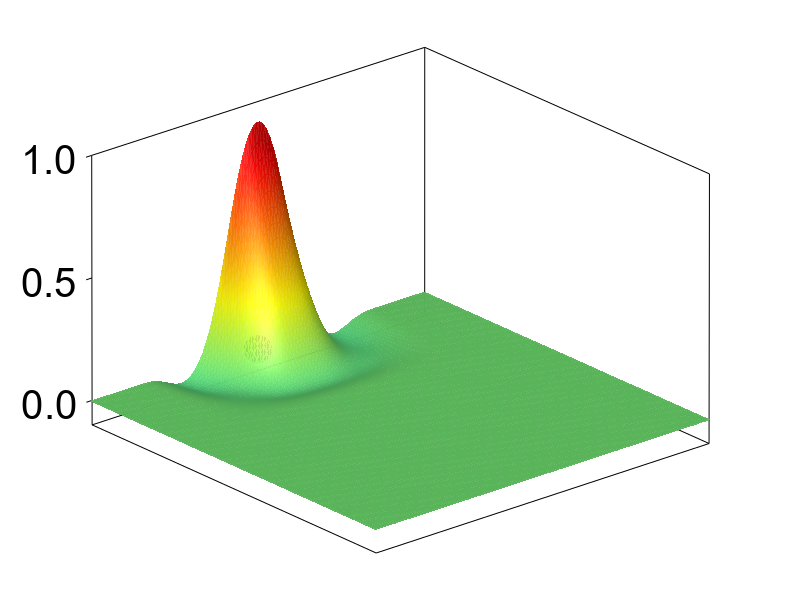
\includegraphics[width=0.7\textwidth]{figures/shape2.png}

                \vspace{-18pt}

                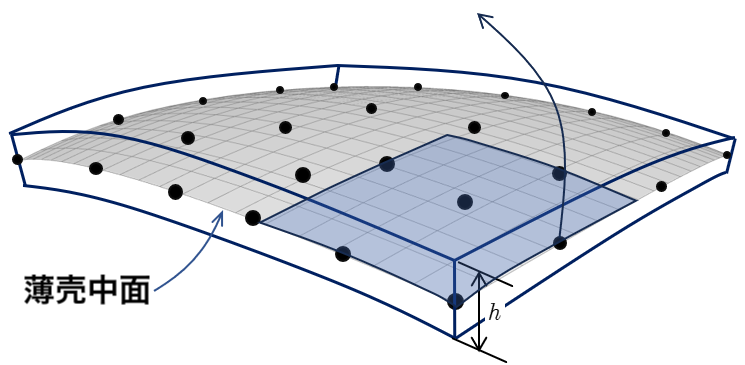
\includegraphics[width=\textwidth]{figures/4.png}
                \caption{\bfseries 边界点处无网格形函数}
            \end{figure}
    
    \end{columns}
\end{frame}

\begin{frame}{无网格形函数高阶导数}
    \begin{columns}
        \column{0.6\textwidth}
        \begin{equation*}
            \Psi_{I,ij}(\boldsymbol{\xi})=\left( \begin{aligned}
            \boldsymbol p_{,ij}^T(\boldsymbol \xi_I-\boldsymbol \xi)\boldsymbol A^{-1}(\boldsymbol \xi)\phi_s(\boldsymbol \xi_I-\boldsymbol \xi)\\
            +\boldsymbol p_{,i}^{T}(\boldsymbol \xi_I-\boldsymbol \xi)\boldsymbol A_{,j}^{-1}(\boldsymbol \xi)\phi_s(\boldsymbol \xi_I-\boldsymbol \xi)\\
            +\boldsymbol p_{,i}^{T}(\boldsymbol \xi_I-\boldsymbol \xi)\boldsymbol A^{-1}(\boldsymbol \xi)\phi_{s,j}(\boldsymbol \xi_I-\boldsymbol \xi)\\
            +\boldsymbol p^{T}(\boldsymbol \xi_I-\boldsymbol \xi)\boldsymbol A_{,ij}^{-1}(\boldsymbol \xi)\phi_s(\boldsymbol \xi_I-\boldsymbol \xi)\\
            +\boldsymbol p_{,j}^{T}(\boldsymbol \xi_I-\boldsymbol \xi)\boldsymbol A_{,i}^{-1}(\boldsymbol \xi)\phi_s(\boldsymbol \xi_I-\boldsymbol \xi)\\
            +\boldsymbol p^{T}(\boldsymbol \xi_I-\boldsymbol \xi)\boldsymbol A_{,i}^{-1}(\boldsymbol \xi)\phi_{s,j}(\boldsymbol \xi_I-\boldsymbol \xi)\\
            +\boldsymbol p^{T}(\boldsymbol \xi_I-\boldsymbol \xi)\boldsymbol A^{-1}(\boldsymbol \xi)\phi_{s,ij}(\boldsymbol \xi_I-\boldsymbol \xi)\\
            +\boldsymbol p_{,j}^{T}(\boldsymbol \xi_I-\boldsymbol \xi)\boldsymbol A^{-1}(\boldsymbol \xi)\phi_{s,i}(\boldsymbol \xi_I-\boldsymbol \xi)\\
            +\boldsymbol p^{T}(\boldsymbol \xi_I-\boldsymbol \xi)\boldsymbol A_{,j}^{-1}(\boldsymbol \xi)\phi_{s,i}(\boldsymbol \xi_I-\boldsymbol \xi)\\
           \end{aligned} \right)
            \boldsymbol p(\boldsymbol 0)
        \end{equation*}

        \column{0.38\textwidth}
            \begin{figure}
                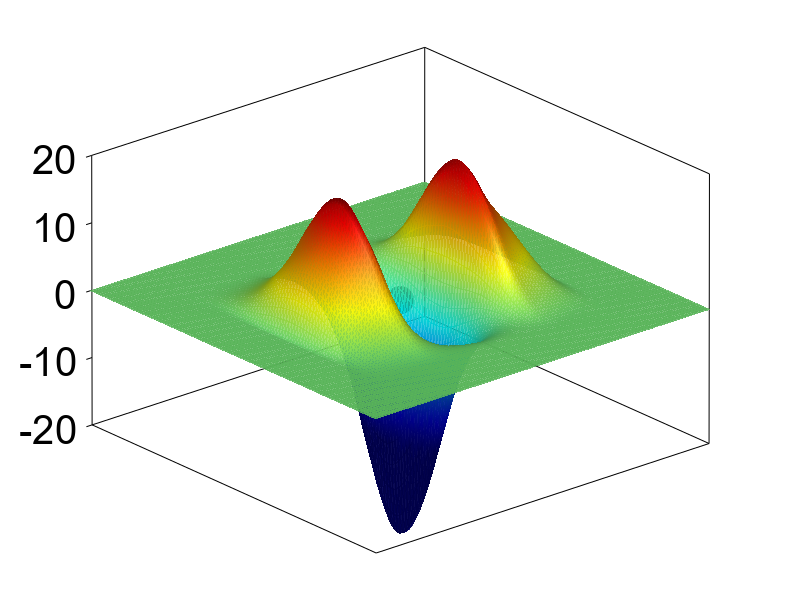
\includegraphics[width=\textwidth]{figures/shape3.png}
                \caption{\bfseries 形函数二阶导数}
            \end{figure}

            \vspace{-20pt}

            \begin{tcolorbox}[colback=red!5, colframe=red!75!black,left=5pt,right=5pt]
                \bfseries\centering 无网格形函数高阶导数\\计算复杂耗时
            \end{tcolorbox}
    \end{columns}

\end{frame}

\section{薄壳问题变分一致性与准变分一致积分方案}

\begin{frame}{薄壳伽辽金法的变分一致性}

\end{frame}
\section{基于 Hu-Washizu 原理变分一致型本质边界条件施加方法}
\begin{frame}{数值算例}
    \begin{columns}
        \column{0.35\textwidth}
            \begin{figure}
                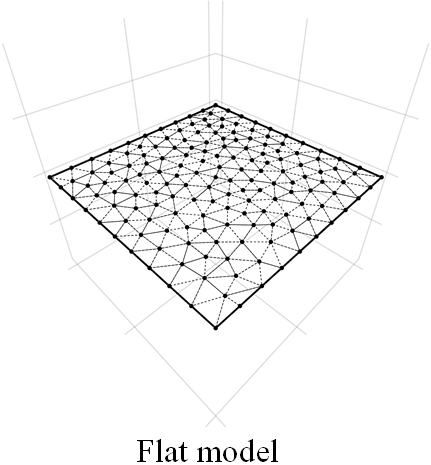
\includegraphics[width=\linewidth, trim=10 0 10 0, clip]{figures/ptmsh1.png}
            \end{figure}

        \column{0.65\textwidth}
            \begin{table}[!ht]
            \centering
            \footnotesize
            \caption{Results of patch test for flat model.}
            \begin{tabular}{lcccc}
            \toprule
            & \multicolumn{2}{c}{Linear patch test} & \multicolumn{2}{c}{Quadratic patch test} \\ \cline{2-5}
            & $L_2$-Error & $H_e$-Error & $L_2$-Error & $H_e$-Error \\
            \midrule
            GI-Penalty & 1.41E-04 & 4.62E-03 & 1.97E-03 & 7.17E-03 \\
            GI-Nitsche & 1.73E-04 & 5.61E-03 & 1.85E-03 & 7.76E-03 \\
            RKGSI-Penalty & 5.04E-09 & 1.02E-07 & 3.01E-09 & 3.41E-08 \\
            RKGSI-Nitsche & 9.75E-12 & 8.98E-11 & 1.29E-12 & 1.06E-12 \\
            RKGSI-HR & 6.15E-13 & 6.91E-12 & 7.51E-13 & 8.36E-12 \\
            \bottomrule
            \end{tabular}
        \end{table}

        \vspace{0.1cm}
        \centering
        \footnotesize
        $\boldsymbol v = \begin{Bmatrix}
        (\xi^1+2\xi^2)^n \\ (3\xi^1+4\xi^2)^n \\ (5\xi^1+6\xi^2)^n
        \end{Bmatrix}$,\quad
        $n = \begin{cases}
        1 & \text{Linear} \\
        2 & \text{Quadratic}
        \end{cases}$
    \end{columns}
\end{frame}


\begin{frame}{数值算例}
    \begin{columns}
        \column{0.35\textwidth}
            \begin{figure}
                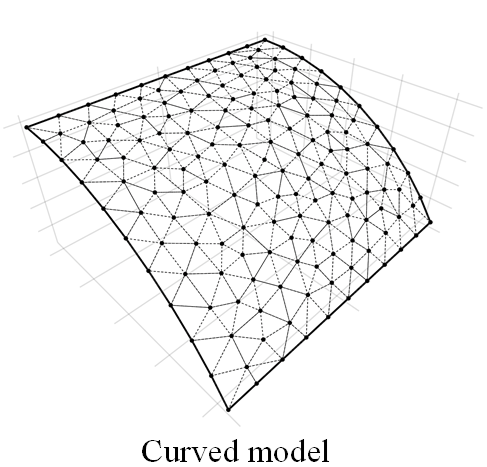
\includegraphics[width=\linewidth, trim=10 0 10 0, clip]{figures/ptmsh.png}
            \end{figure}

        \column{0.65\textwidth}
            \begin{table}[!ht]
            \footnotesize
            \centering
            \caption{Results of patch test for cylindrical model.}\label{ptt2}
            \begin{tabular}{lcccc}
            \toprule
            & \multicolumn{2}{c}{Linear patch test} & \multicolumn{2}{c}{Quadratic patch test} \\ \cline{2-5}
            & $L_2$-Error & $H_e$-Error & $L_2$-Error & $H_e$-Error \\
            \midrule
            GI-Penalty & 1.75E-04 & 4.50E-03 & 1.08E-03 & 5.83E-03 \\
            GI-Nitsche & 1.77E-04 & 5.36E-03 & 1.07E-03 & 6.33E-03 \\
            RKGSI-Penalty & 8.59E-05 & 9.11E-04 & 4.28E-04 & 2.08E-03 \\
            RKGSI-Nitsche & 1.27E-05 & 5.32E-05 & 1.88E-05 & 5.6E-04 \\
            RKGSI-HR & 1.43E-05 & 1.60E-04 & 2.93E-05 & 2.85E-04 \\
            \bottomrule
        \end{tabular}
        \end{table}

        \vspace{0.1cm}
        \centering
        \footnotesize
        $\boldsymbol v = \begin{Bmatrix}
        (\xi^1+2\xi^2)^n \\ (3\xi^1+4\xi^2)^n \\ (5\xi^1+6\xi^2)^n
        \end{Bmatrix}$,\quad
        $n = \begin{cases}
        1 & \text{Linear} \\
        2 & \text{Quadratic}
        \end{cases}$
    \end{columns}
\end{frame}

\begin{frame}{数值算例}
    \begin{columns}
        \column{0.35\textwidth}
            \begin{figure}
                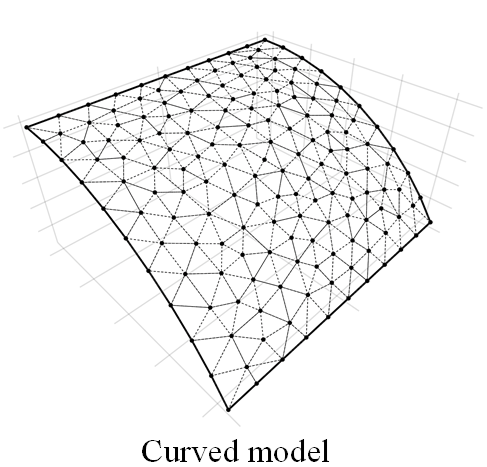
\includegraphics[width=\linewidth, trim=10 0 10 0, clip]{figures/ptmsh.png}
            \end{figure}
        \column{0.65\textwidth}
            \begin{figure}
                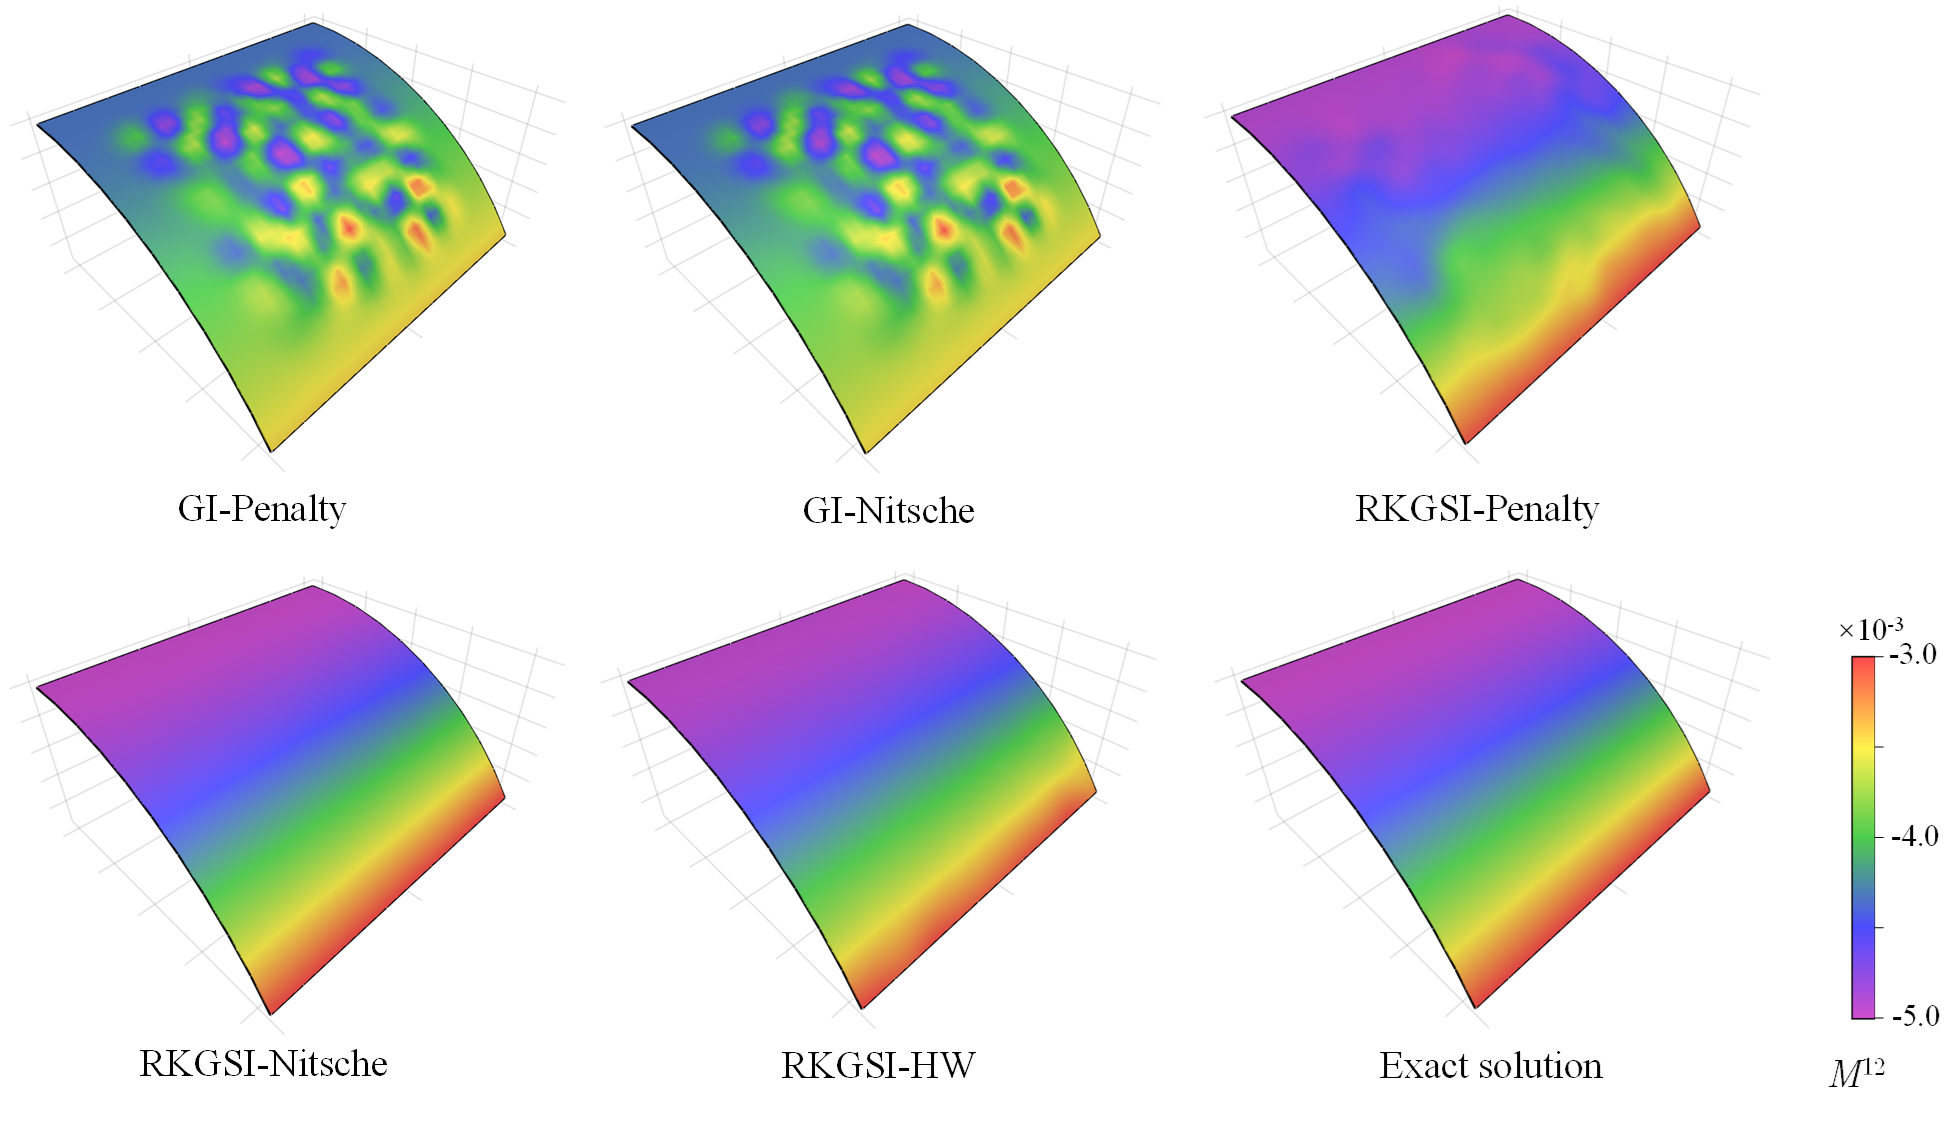
\includegraphics[width=\linewidth, trim=15 10 10 0, clip]{figures/ptc_r2.png}
                \caption{曲壳分片试验$M^{12}$云图}
            \end{figure}
    \end{columns}
\end{frame}

\begin{frame}{数值算例}
    \begin{columns}
        \column{0.4\textwidth}
            \begin{figure}
                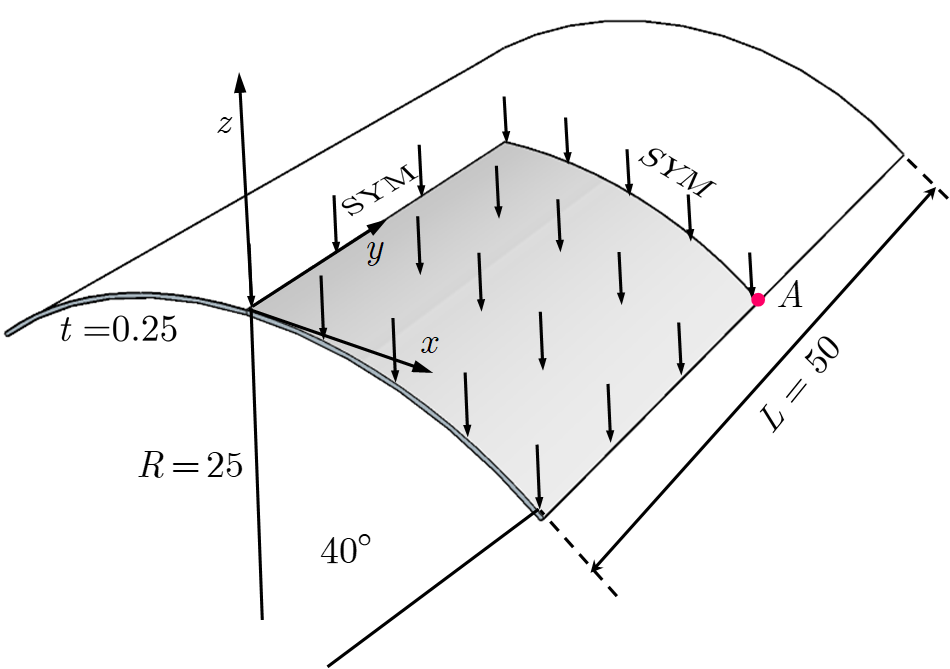
\includegraphics[height=0.7\textwidth]{figures/slm.png}
                \caption{Scordelis-Lo 屋顶问题描述}

                \centering
                \small
                {\color{myblue}
                \fbox{
                \begin{tabular}{@{} l @{\quad} l @{}}
                    \textbf{杨氏模量} & $E = 4.32 \times 10^8$ \\[0.8em]
                    \textbf{泊松比}   & $\nu = 0.0$           \\[0.8em]
                    \textbf{荷载}     & $q = 90.0$
                \end{tabular}
                }}
            \end{figure}
        \column{0.55\textwidth}
            \begin{figure}
                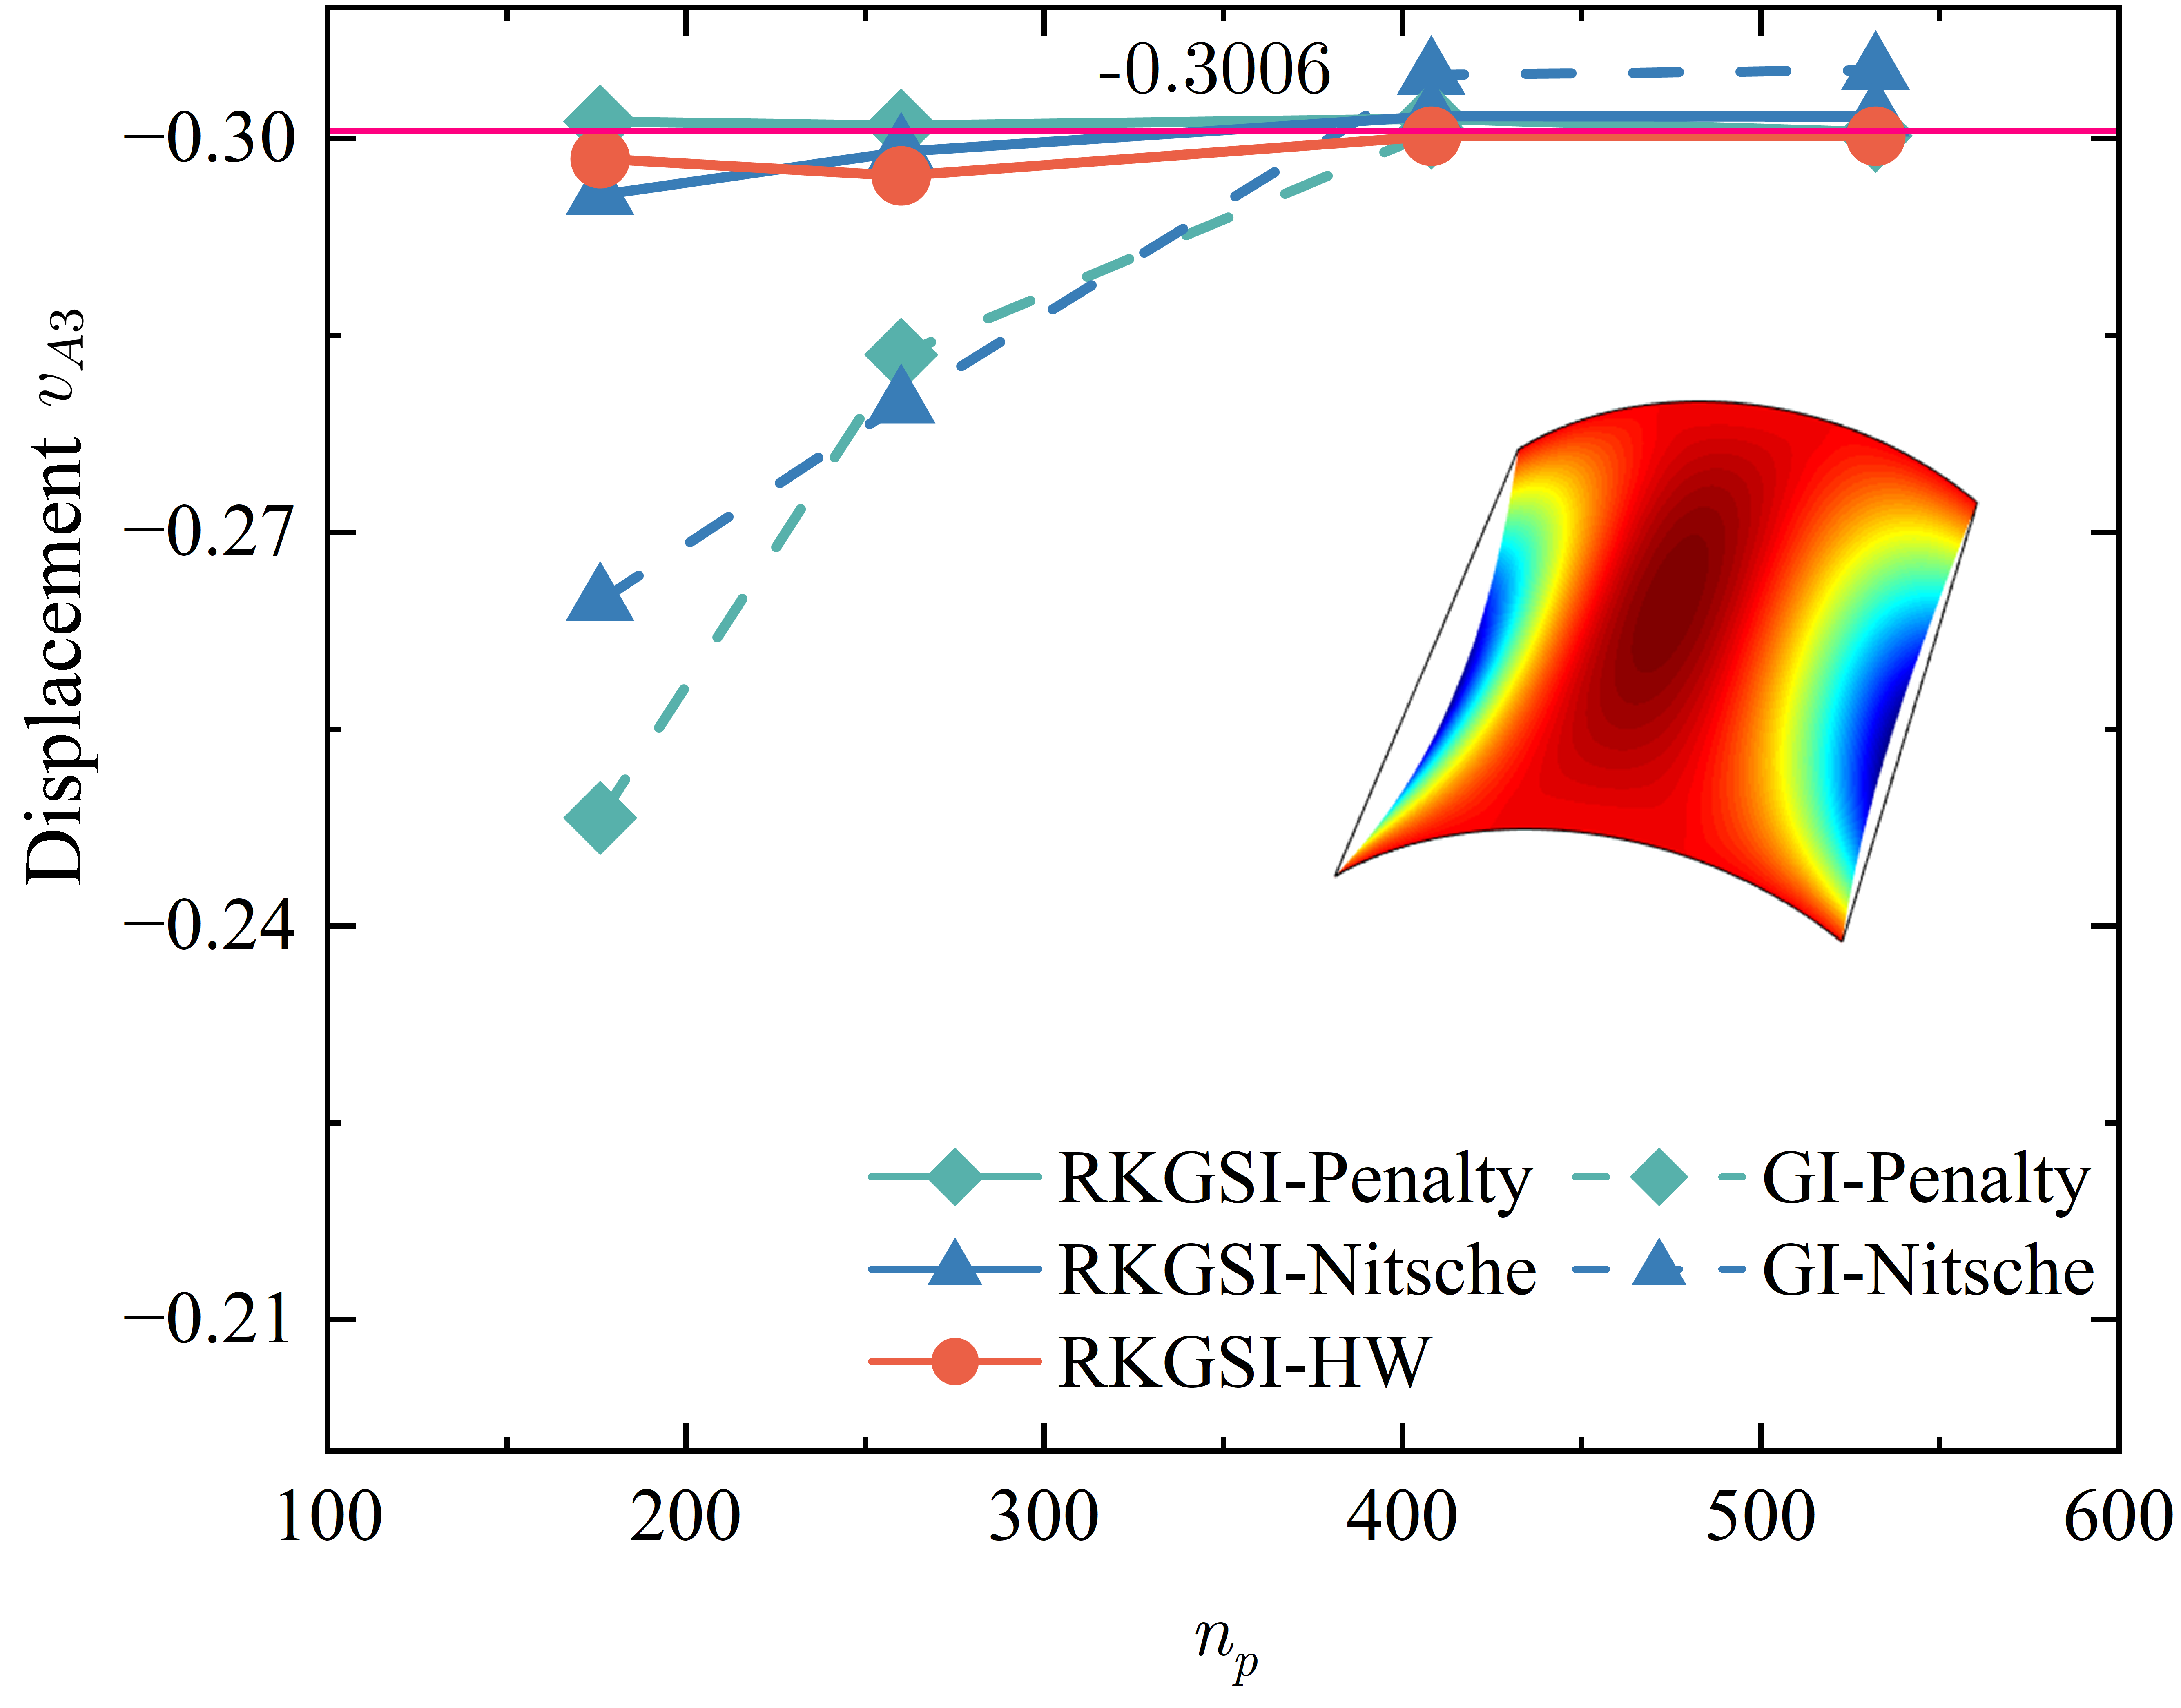
\includegraphics[height=0.7\textwidth]{figures/sld_r2.png}
                \caption{Scordelis-Lo屋顶问题的位移收敛性}
            \end{figure}
    \end{columns}
\end{frame}

\begin{frame}{数值算例}
\begin{figure}[htbp]
    \centering 
    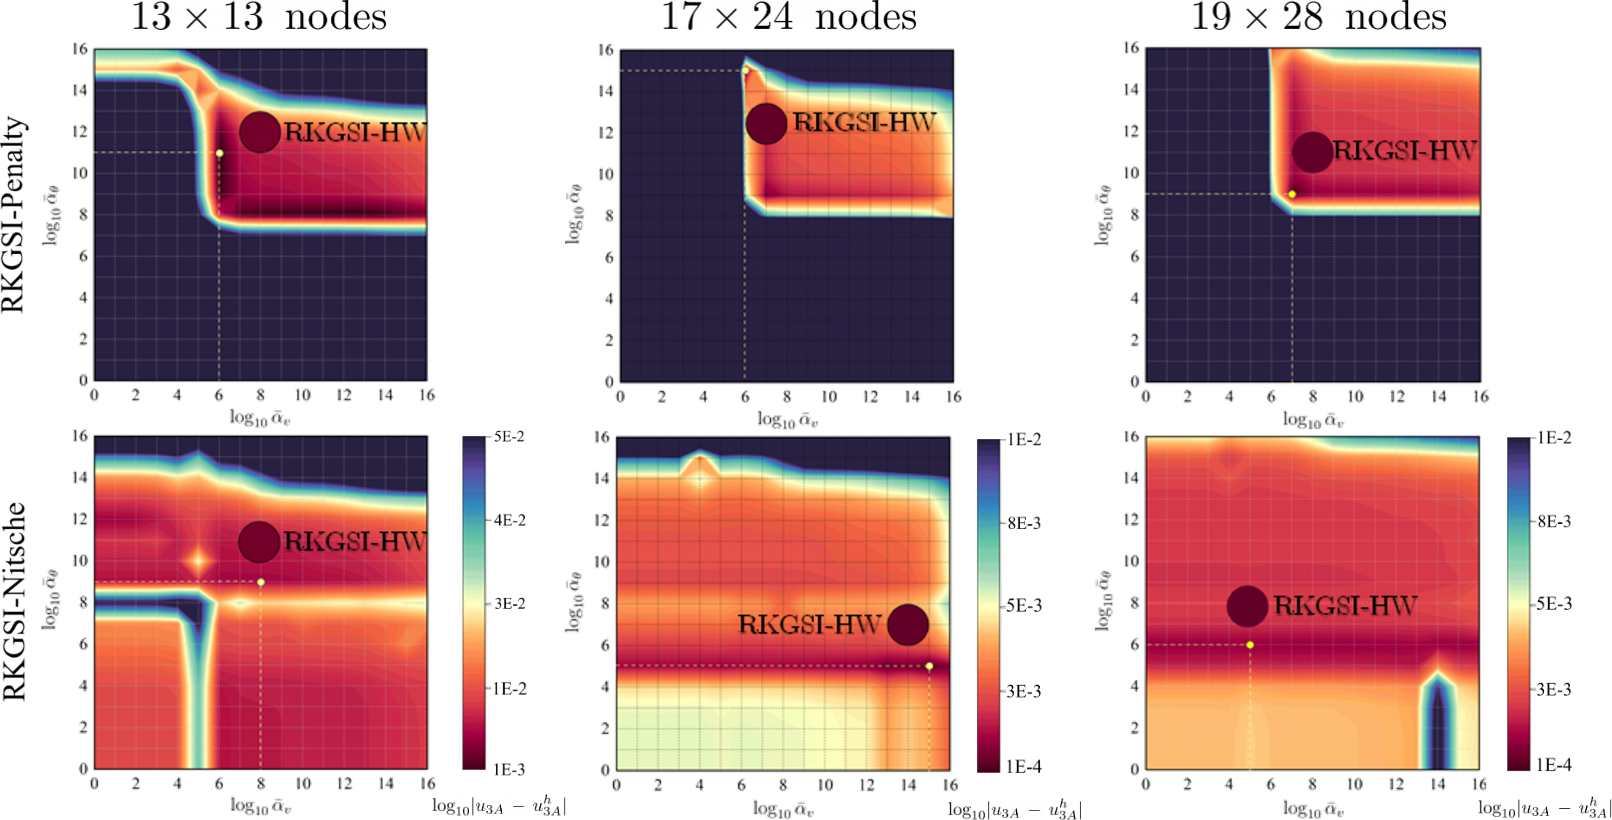
\includegraphics[width=0.85\textwidth]{figures/RKGSI.png}
    \caption{Scordelis‑Lo 屋顶问题中参数$\alpha_v$和$\alpha_\theta$的灵敏度对比}
\end{figure}
\end{frame}

\begin{frame}{数值算例}
    \begin{columns}
        \column{0.4\textwidth}
            \begin{figure}
                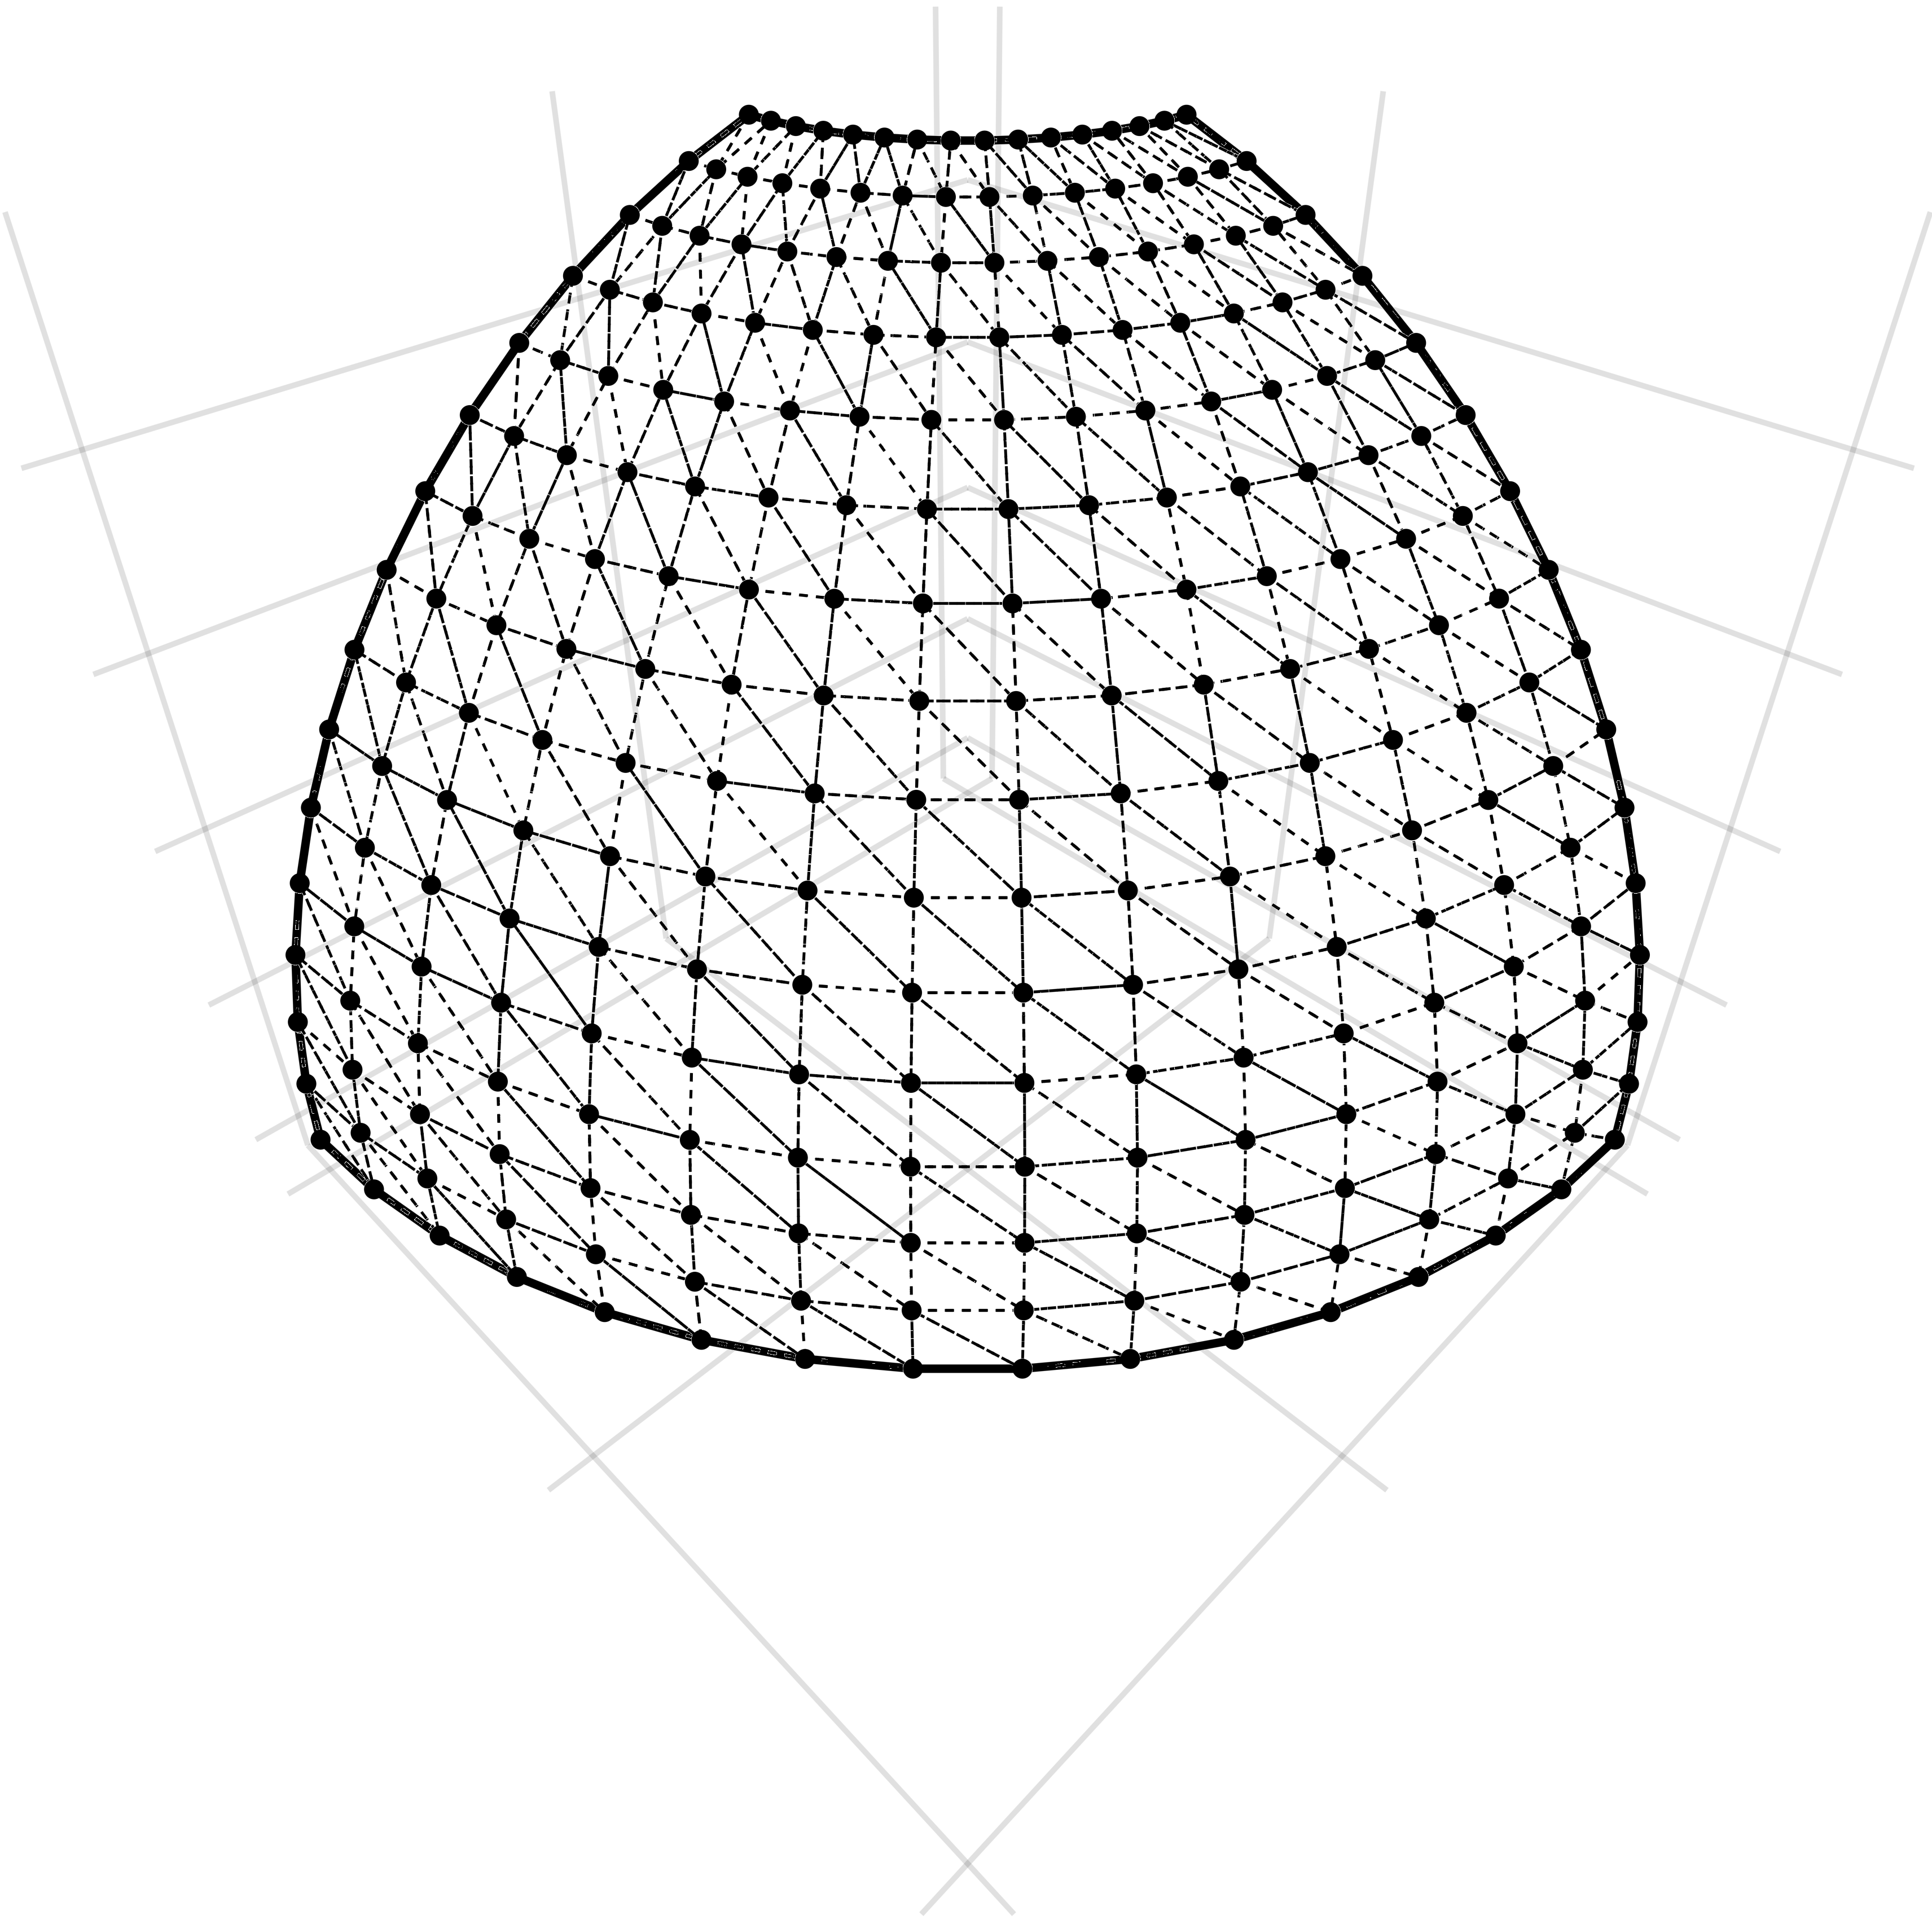
\includegraphics[width=\linewidth, trim=50 0 50 0, clip]{figures/sphericalshell_16.png}
                \caption{曲壳屋顶问题}
            \end{figure}
        \column{0.55\textwidth}
            \begin{figure}
                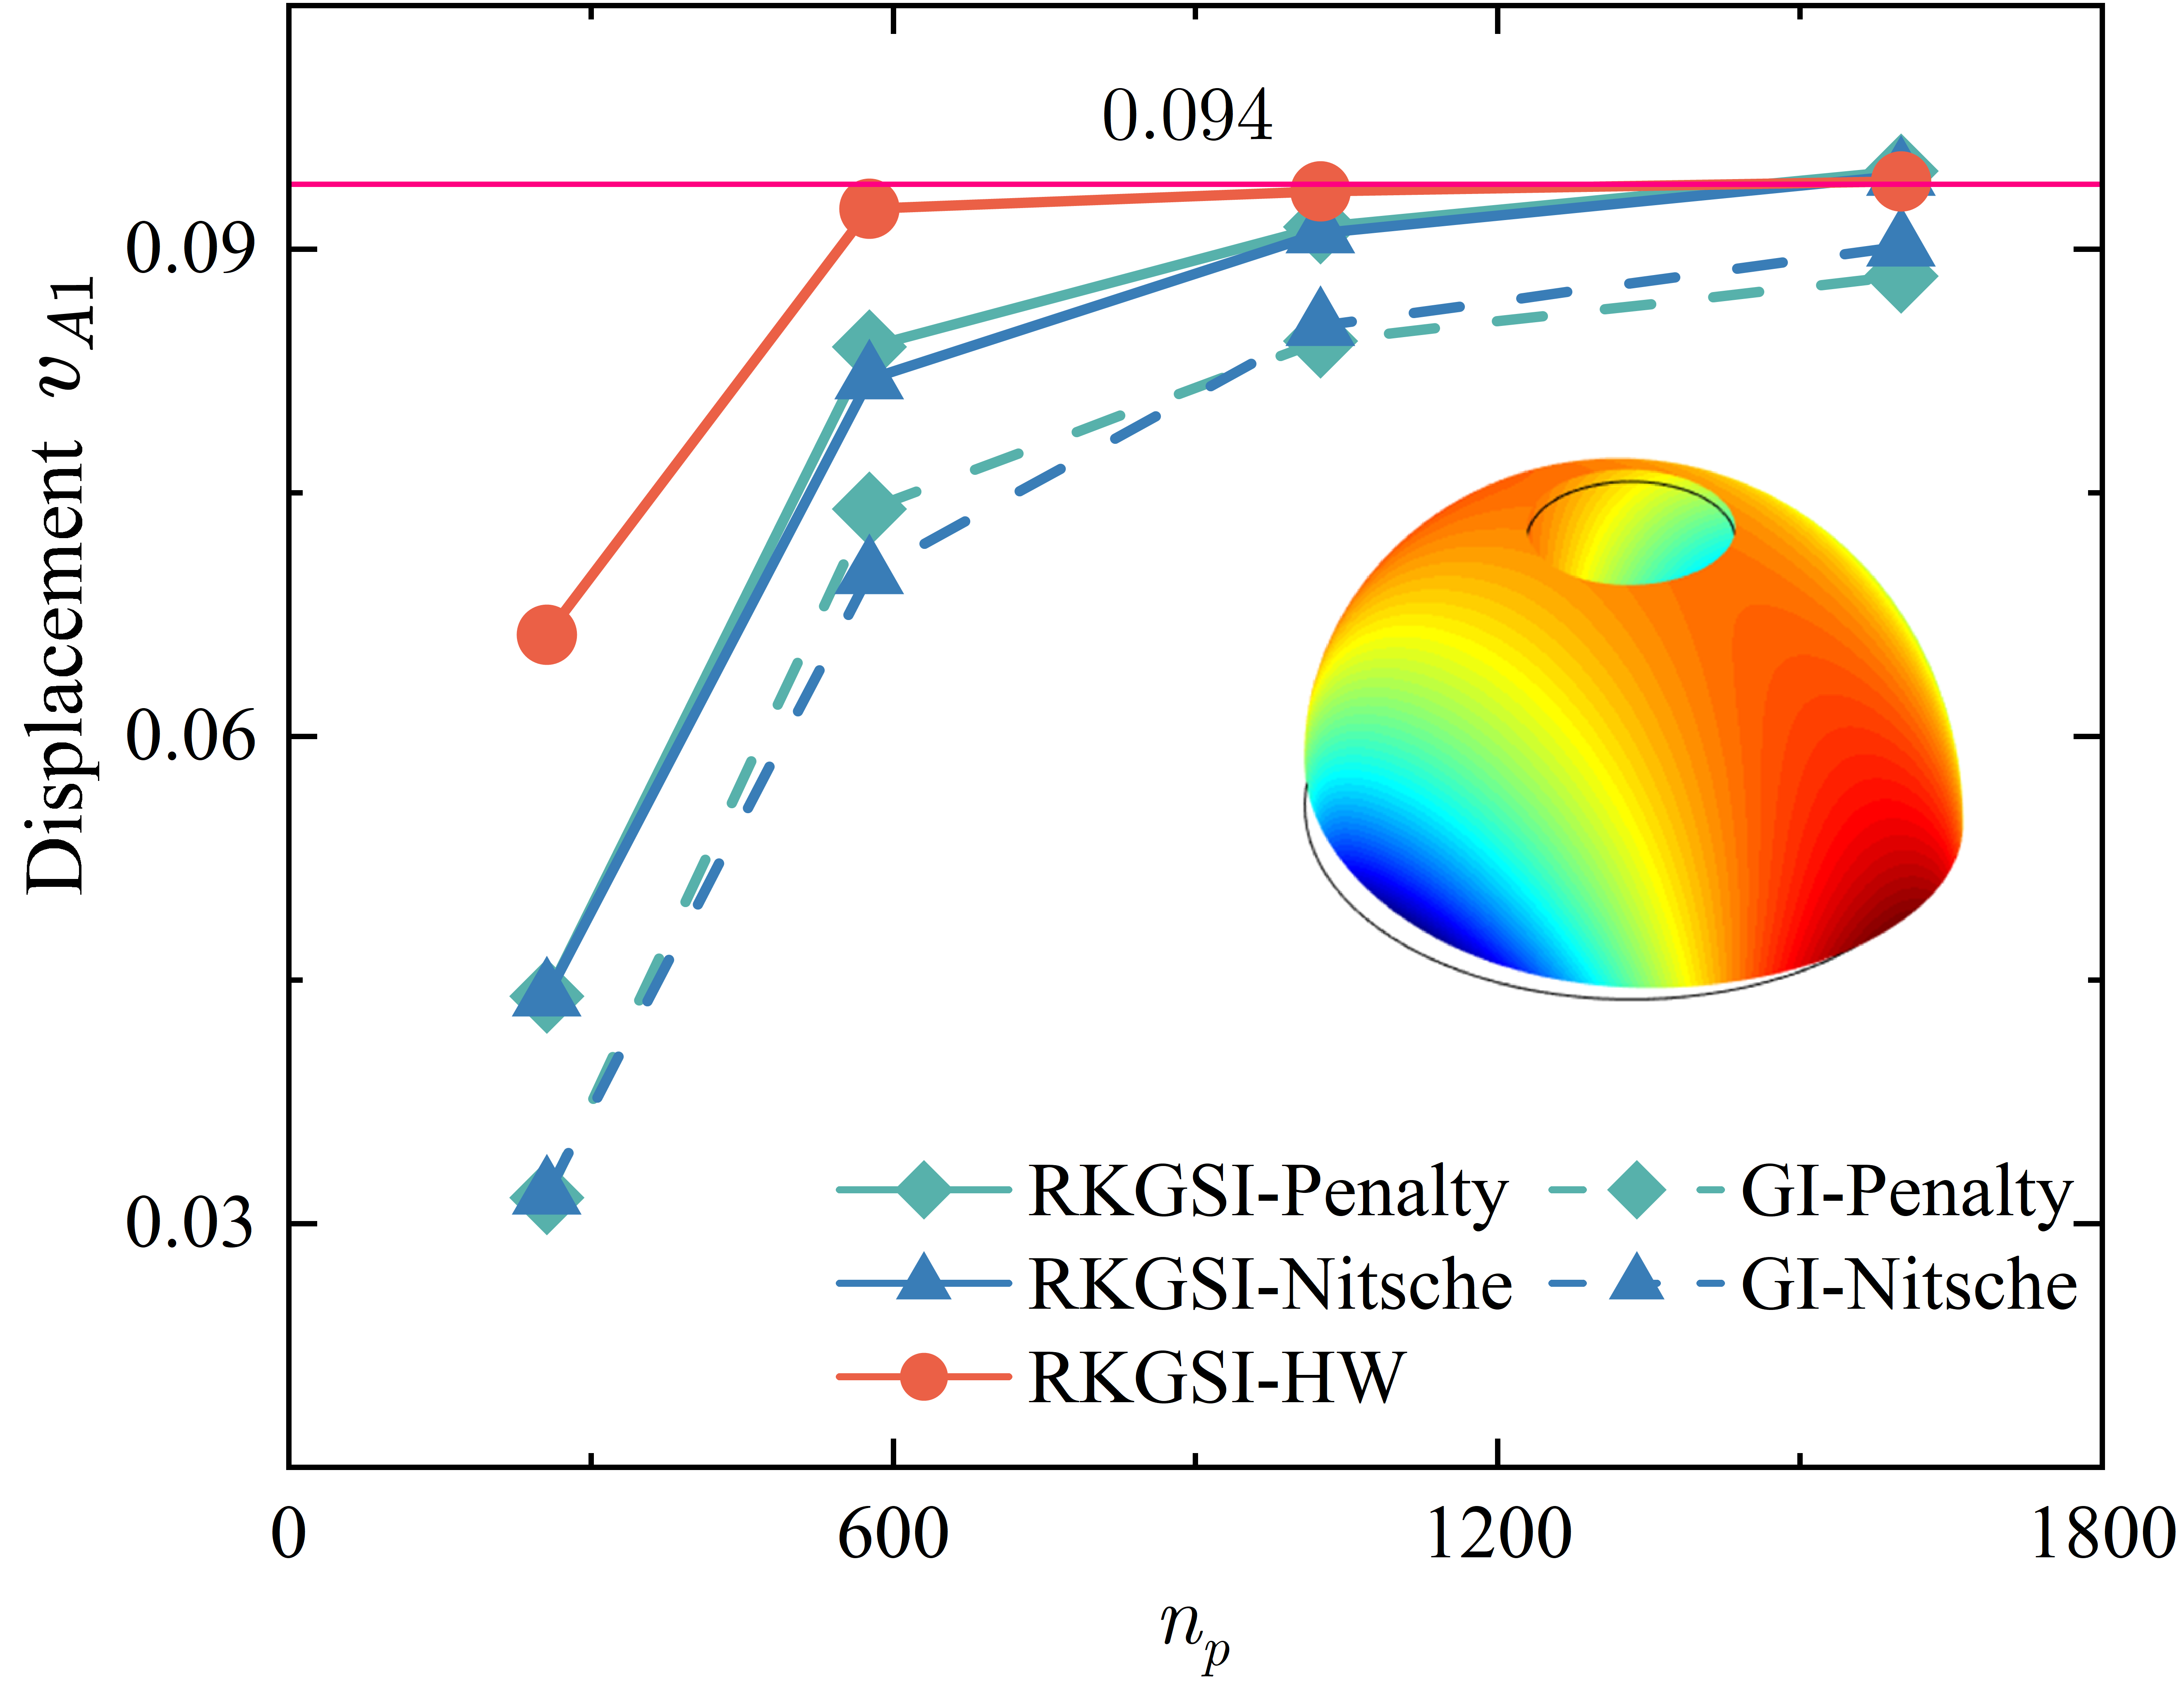
\includegraphics[height=0.7\textwidth]{figures/pfd_r1.png}
                \caption{球壳问题}
            \end{figure}
    \end{columns}
\end{frame}

\begin{frame}{数值算例}
    \begin{columns}
        \column{0.4\textwidth}
            \begin{figure}
                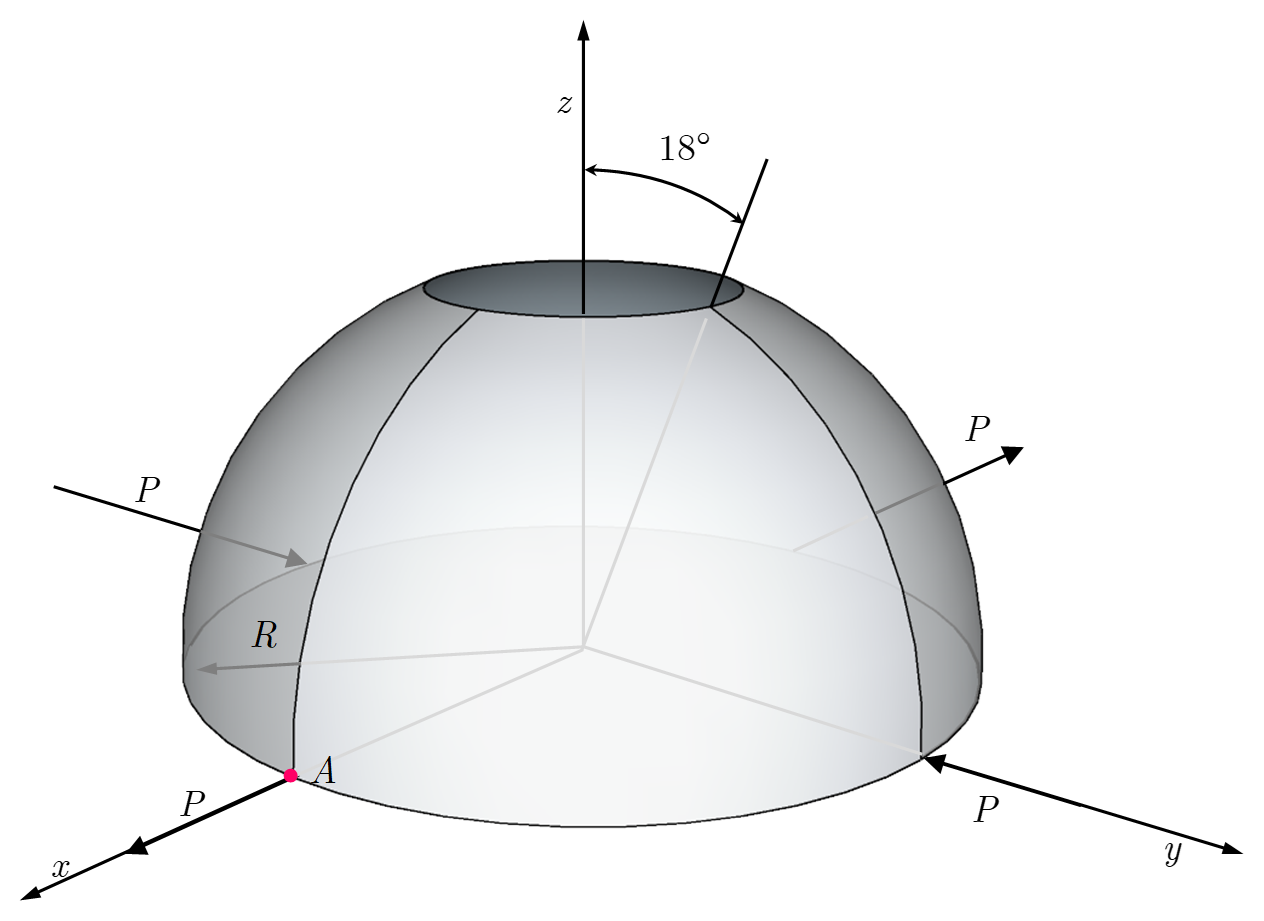
\includegraphics[width=\linewidth, trim=50 0 50 0, clip]{figures/pfm.png}
            \end{figure}
        \column{0.55\textwidth}
            \begin{figure}
                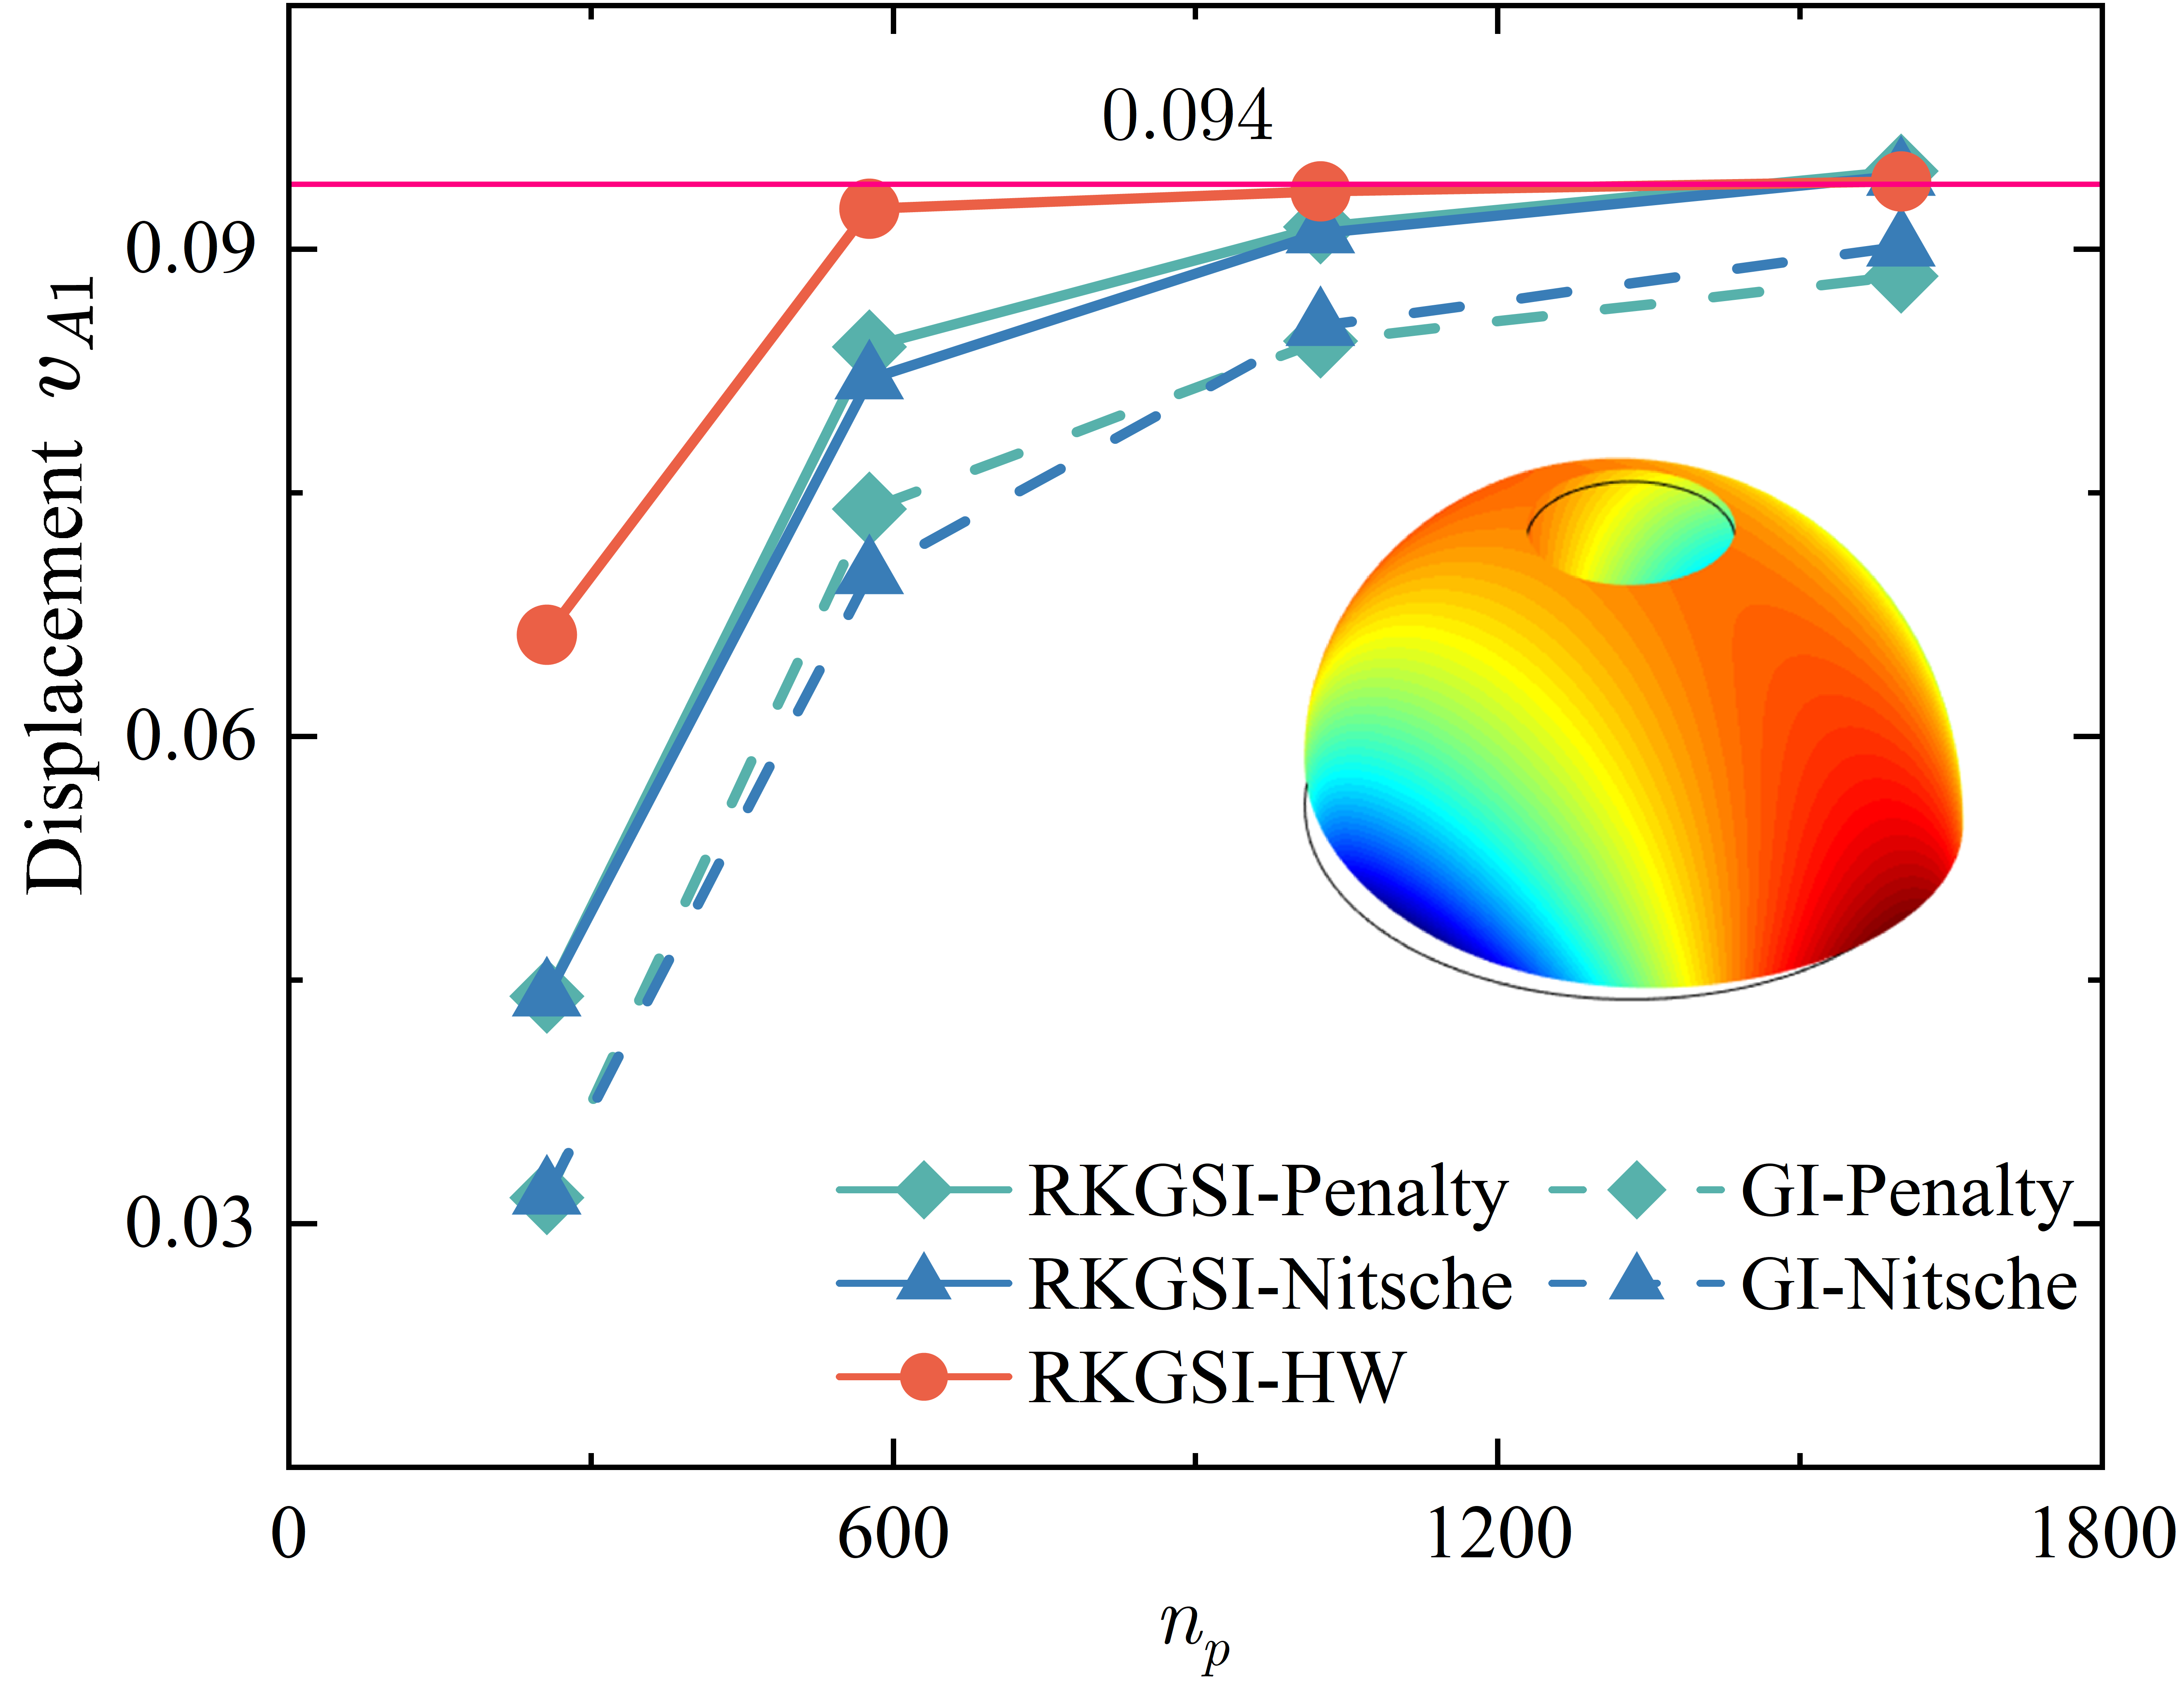
\includegraphics[height=0.7\textwidth]{figures/pfd_r1.png}
            \end{figure}
    \end{columns}

    \vspace{0.1cm}
    \centering
    \footnotesize
    \text{球壳问题}
\end{frame}

\begin{frame}{数值算例}
\begin{figure}[htbp]
    \centering 
    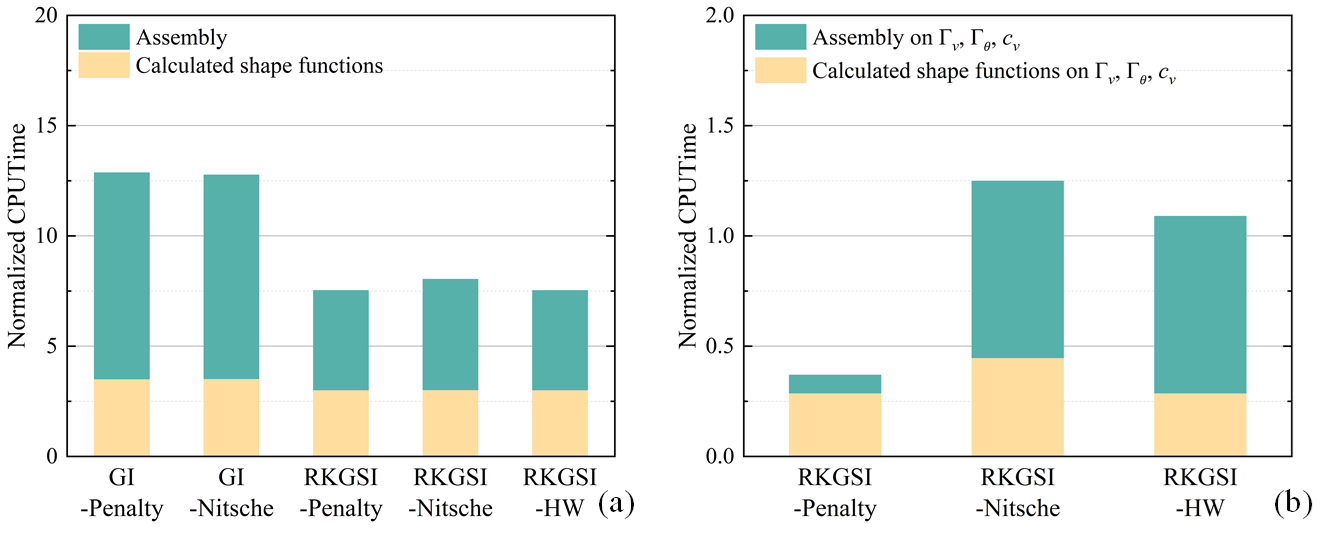
\includegraphics[width=0.95\textwidth]{figures/efficient.png}
    \caption{受压半球壳问题之效率比较：(a) 全域；(b) 本质边界}
\end{figure}
\end{frame}
\section{结论}
\begin{frame}{结论}

\end{frame}

\begin{frame}[plain]

    \centering
    
\includegraphics[height=2cm]{logos/logo1.pdf}
    \quad
    
\includegraphics[height=2cm]{logos/logo2.pdf}

    \vspace{1cm}

    \centering
    \Huge \textbf{谢谢!}
  
\end{frame}


\end{document}